% !TEX root = ../main.tex

%%% ============================================================
\section{Phương pháp HSGE}
%%% ============================================================

\begin{frame}{Tổng quan pipeline HSGE}
  \begin{center}
    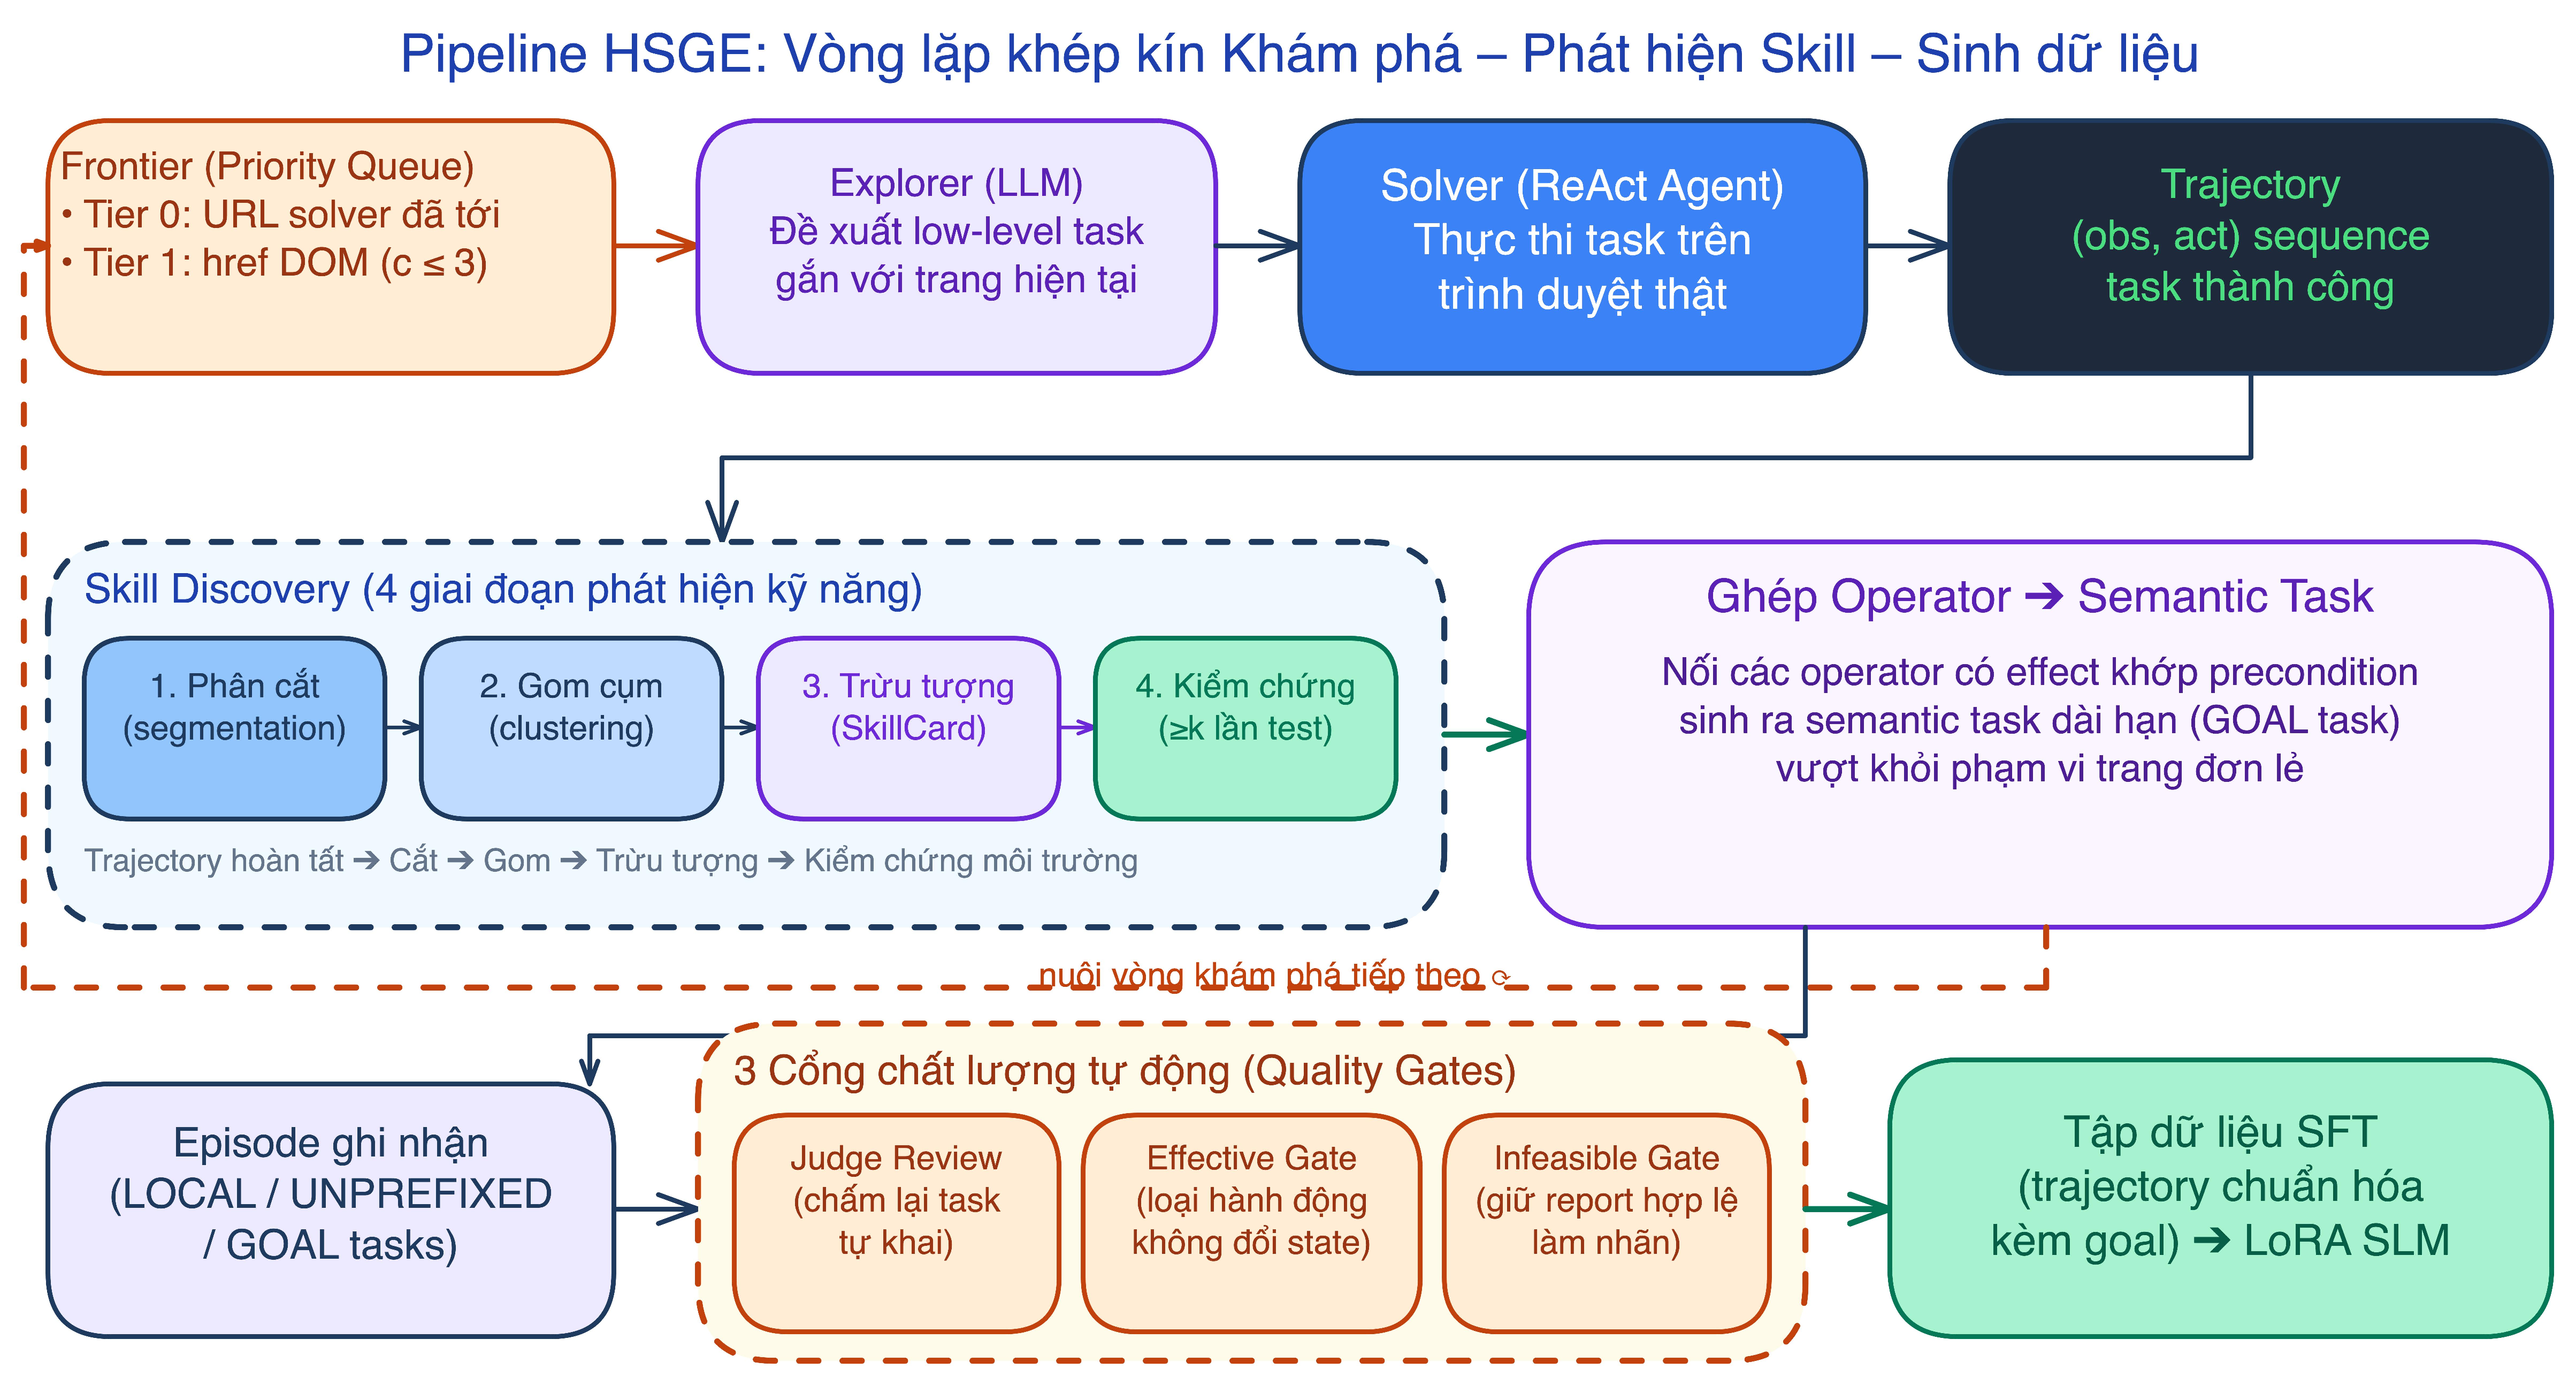
\includegraphics[width=\linewidth,height=0.70\textheight,keepaspectratio]{fig_pipeline.pdf}
  \end{center}
  \figcap{Vòng lặp khép kín: khám phá $\rightarrow$ phát hiện \textbf{skill}
  $\rightarrow$ nâng thành \textbf{operator} $\rightarrow$ ghép chuỗi thành
  \textbf{semantic task}; tri thức thu được lại nuôi vòng khám phá kế tiếp.}
\end{frame}

\begin{frame}{Biểu diễn: đồ thị hai tầng}
  \begin{columns}[c]
    \begin{column}{0.62\textwidth}
      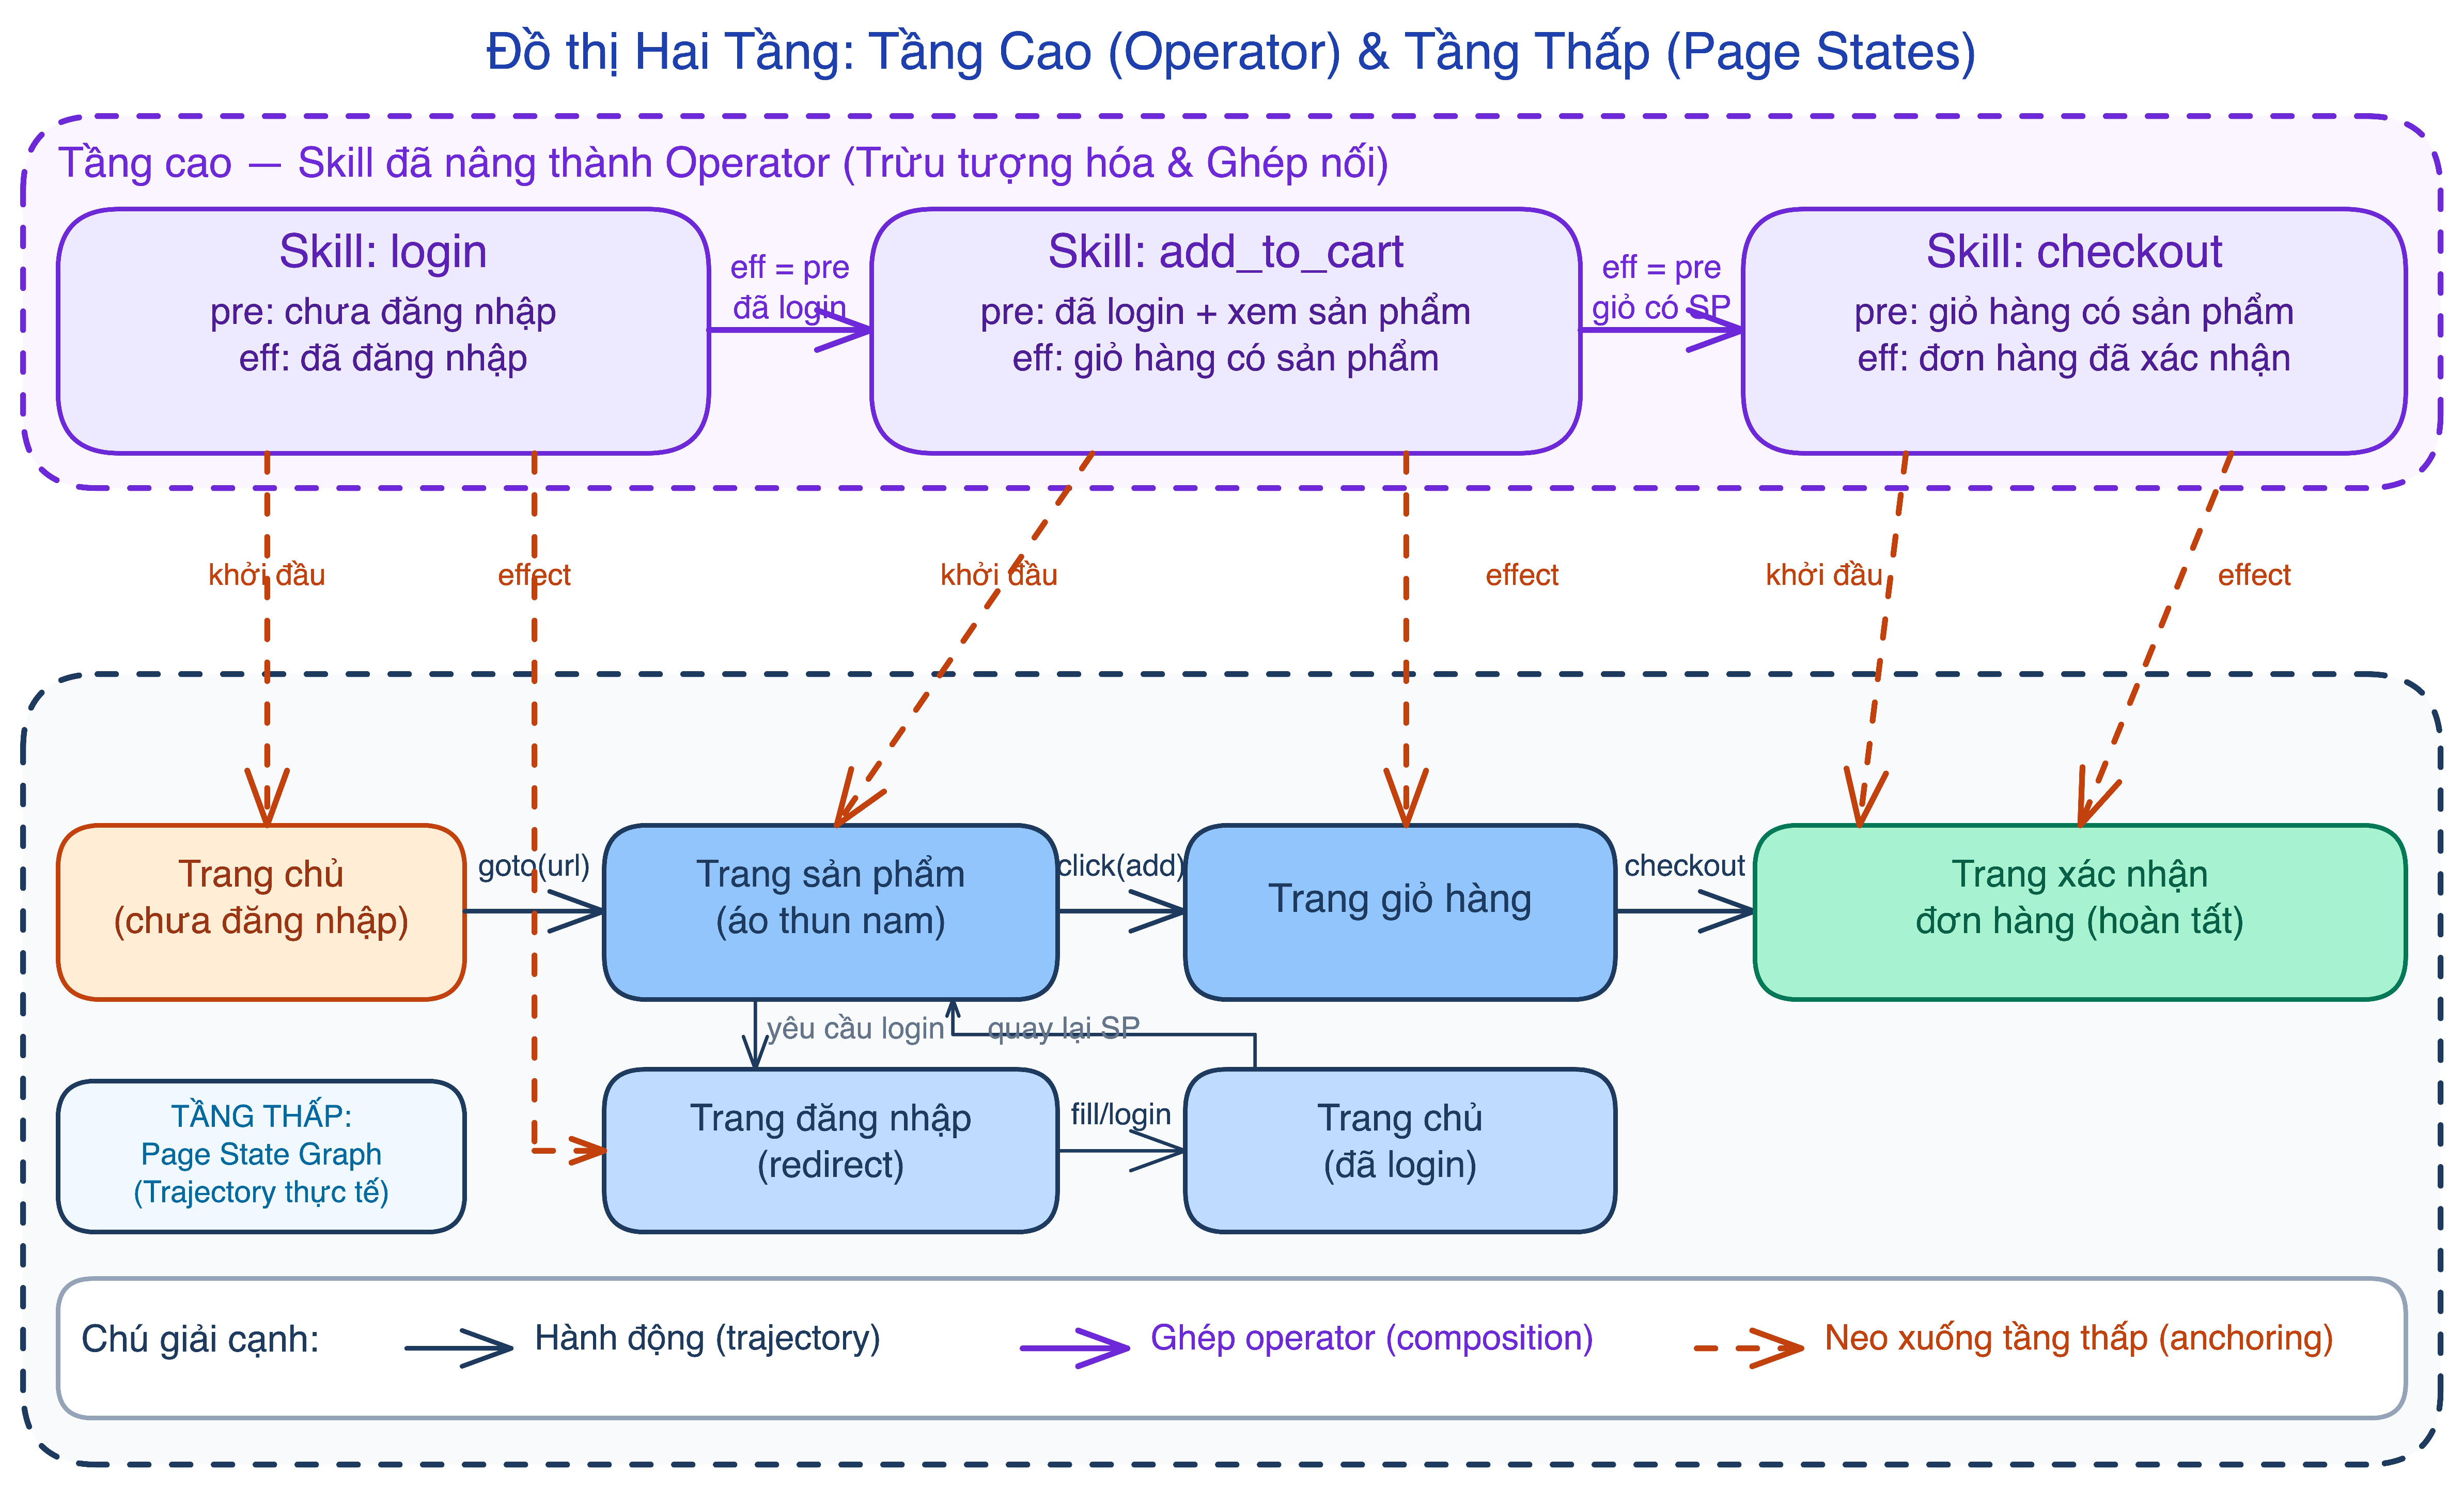
\includegraphics[width=\linewidth,height=0.72\textheight,keepaspectratio]{fig_twolevel.pdf}
    \end{column}
    \begin{column}{0.36\textwidth}
      \footnotesize
      \textbf{Tầng thấp} --- trạng thái trang đã thăm, nối bởi cạnh hành động
      (website mô hình hóa như một POMDP).

      \vspace{0.25cm}
      \textbf{Tầng cao} --- skill dưới dạng \emph{option} $\langle I,\pi,\beta\rangle$,
      được nâng thành \textbf{operator} mang \emph{precondition} và \emph{effect}
      phát biểu bằng ngôn ngữ tự nhiên đã chuẩn hóa.

      \vspace{0.25cm}
      Hai operator nối được với nhau khi \kw{effect} của cái trước
      \kw{thỏa precondition} của cái sau --- đây chính là cạnh sinh ra
      task dài hạn.

      \vspace{0.25cm}
      \textit{Hệ quả:} tri thức khám phá được lưu ở dạng
      \emph{tái sử dụng và tái tổ hợp được}, không phải một đống trajectory rời rạc.
    \end{column}
  \end{columns}
\end{frame}

\begin{frame}{Khám phá có định hướng: frontier hai tầng}
  \begin{columns}[c]
    \begin{column}{0.63\textwidth}
      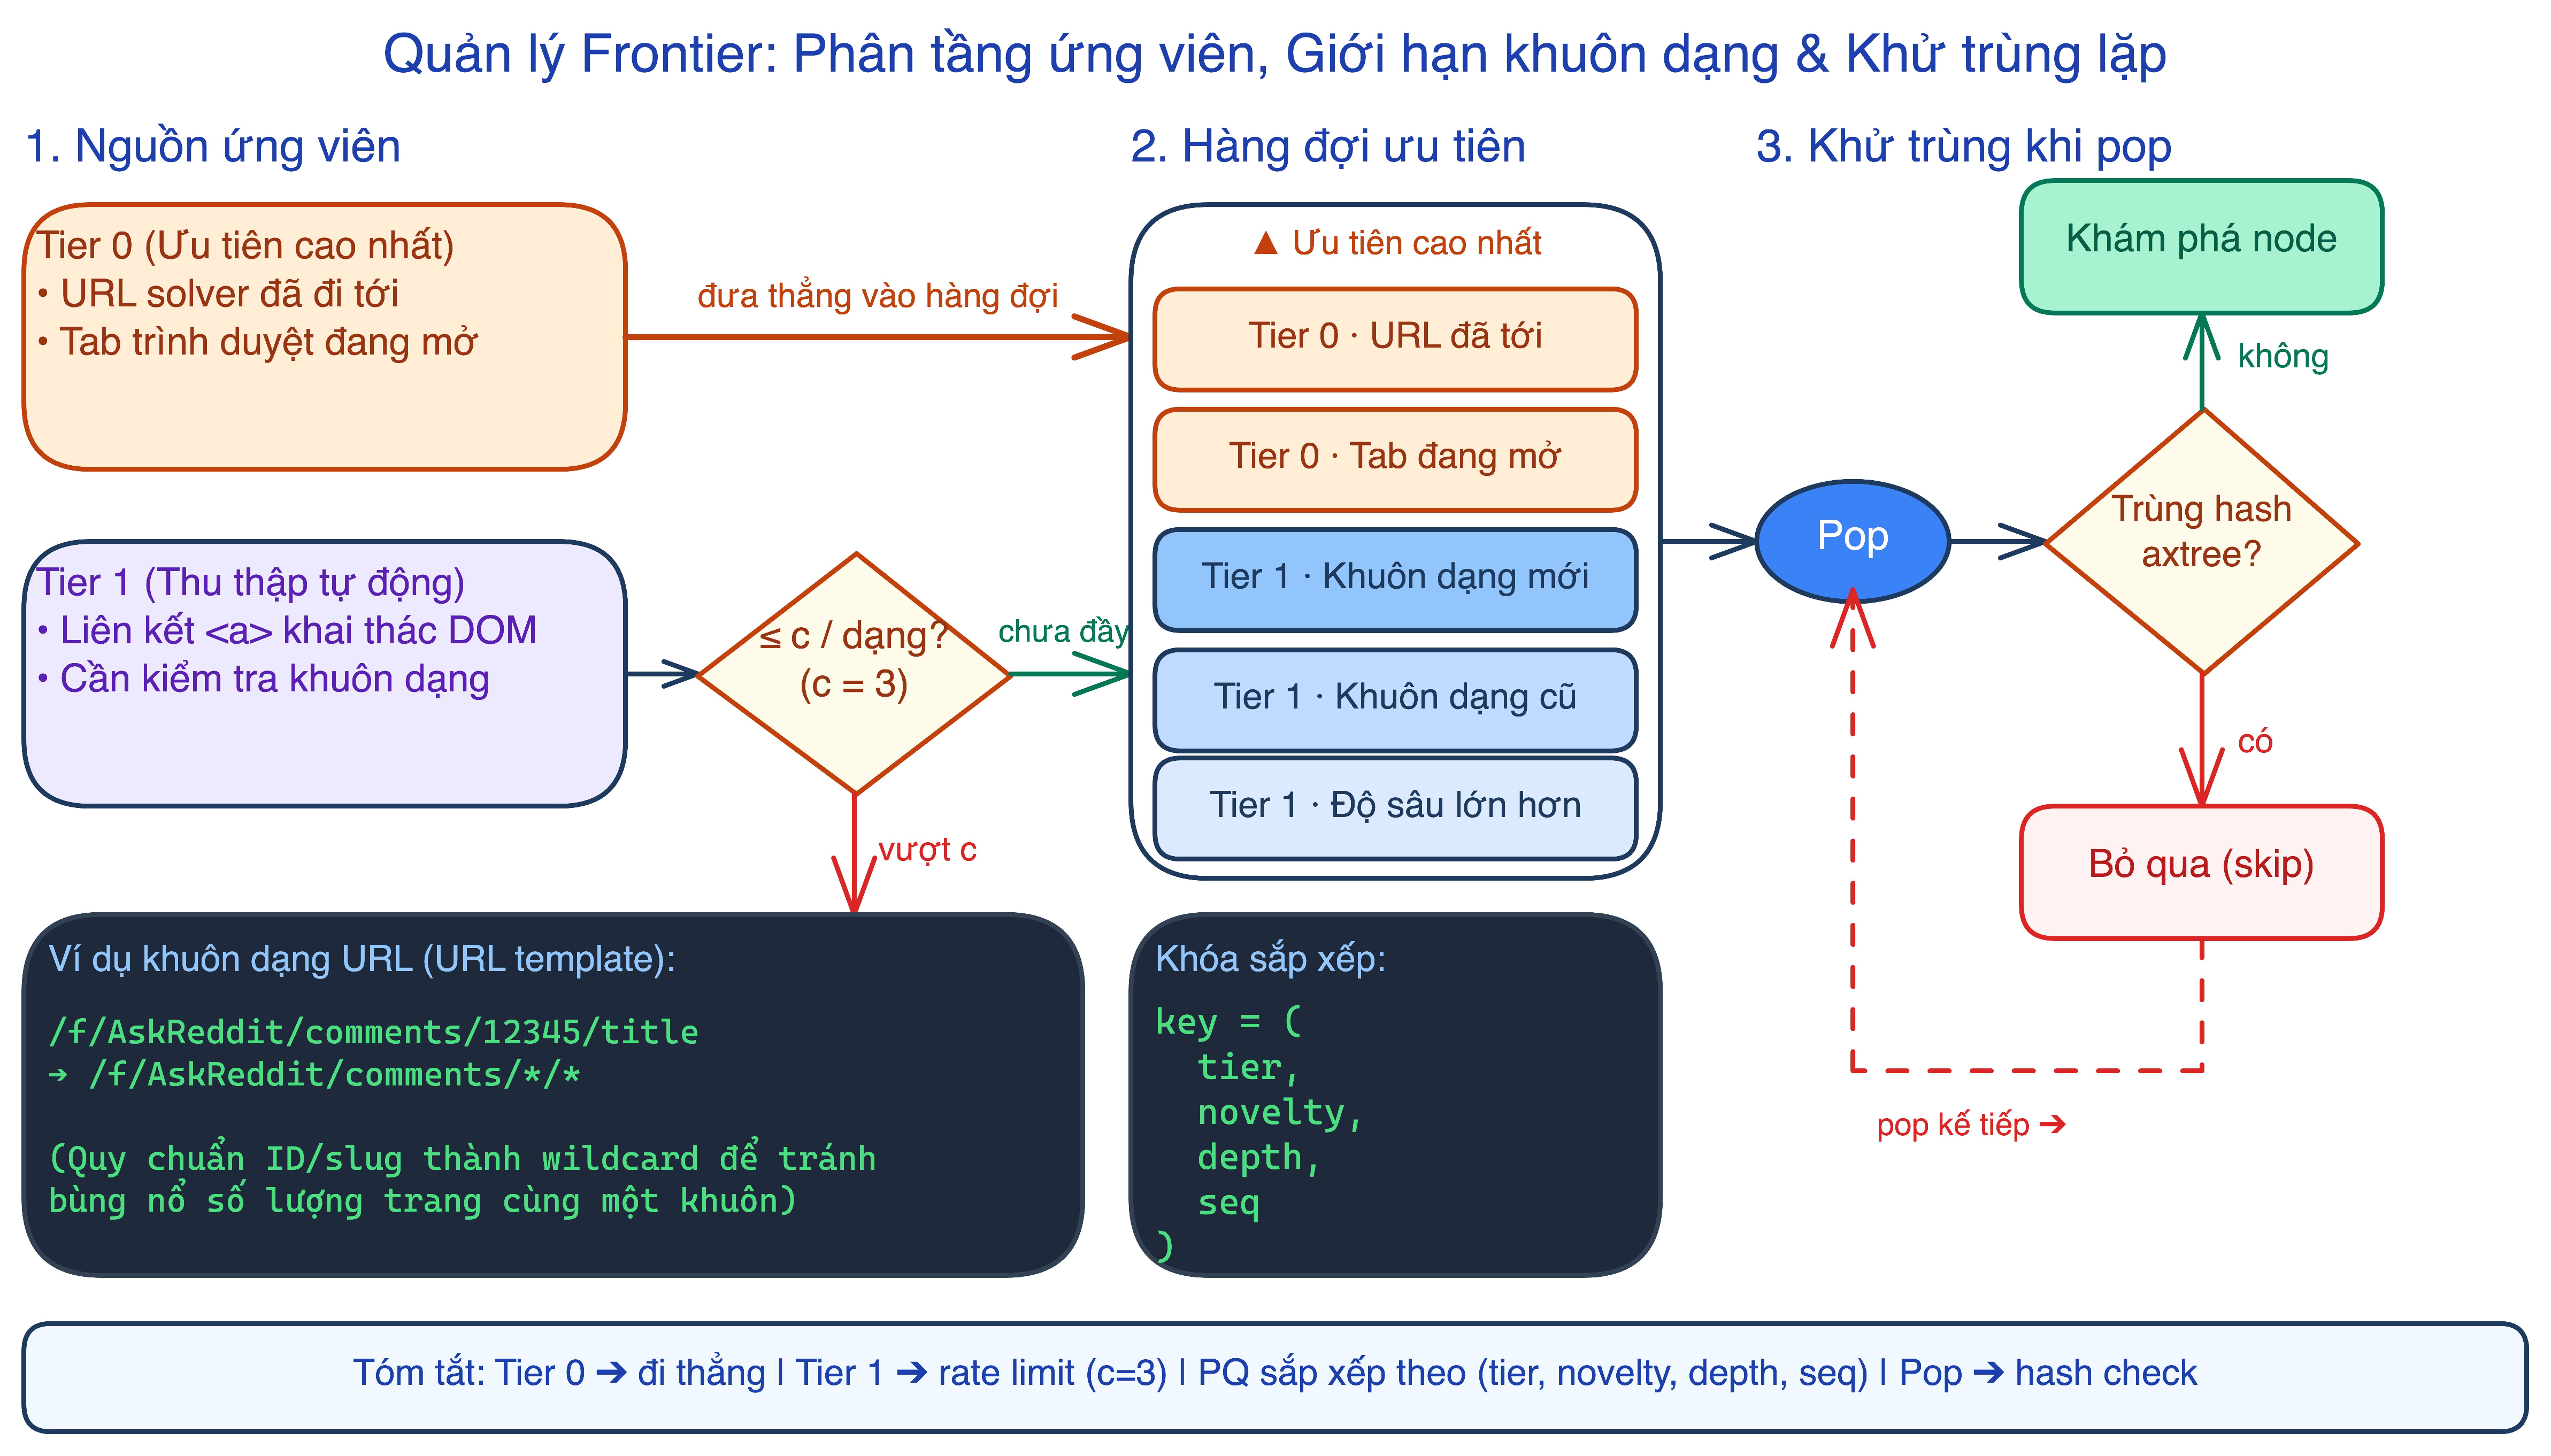
\includegraphics[width=\linewidth,height=0.70\textheight,keepaspectratio]{fig_frontier.pdf}
    \end{column}
    \begin{column}{0.35\textwidth}
      \footnotesize
      \textbf{Tier 0} --- URL solver đã thực sự đi tới: vào thẳng hàng đợi.

      \textbf{Tier 1} --- liên kết khai thác từ DOM: phải qua
      \emph{giới hạn theo khuôn dạng URL} ($\le 3$ trang/khuôn dạng), nên
      hàng nghìn trang sản phẩm hay bài đăng không thể làm ngập frontier.

      \vspace{0.2cm}
      Ưu tiên: \emph{tầng} $\rightarrow$ \emph{độ mới của khuôn dạng}
      $\rightarrow$ \emph{độ sâu}. Node có nội dung trùng mã băm với trang đã
      thăm thì bị bỏ qua (\kw{31/258} node).

      \vspace{0.2cm}
      \textbf{Solver} có chốt chặn cấu trúc thay vì chỉ nhắc bằng prompt:
      cảnh báo rồi \emph{dừng cứng} khi lặp cùng một đích mà trang không đổi;
      \texttt{report\_infeasible} là kết cục hợp lệ.
    \end{column}
  \end{columns}
\end{frame}

\begin{frame}{Phát hiện skill và quy nạp operator}
  \begin{columns}[c]
    \begin{column}{0.40\textwidth}
      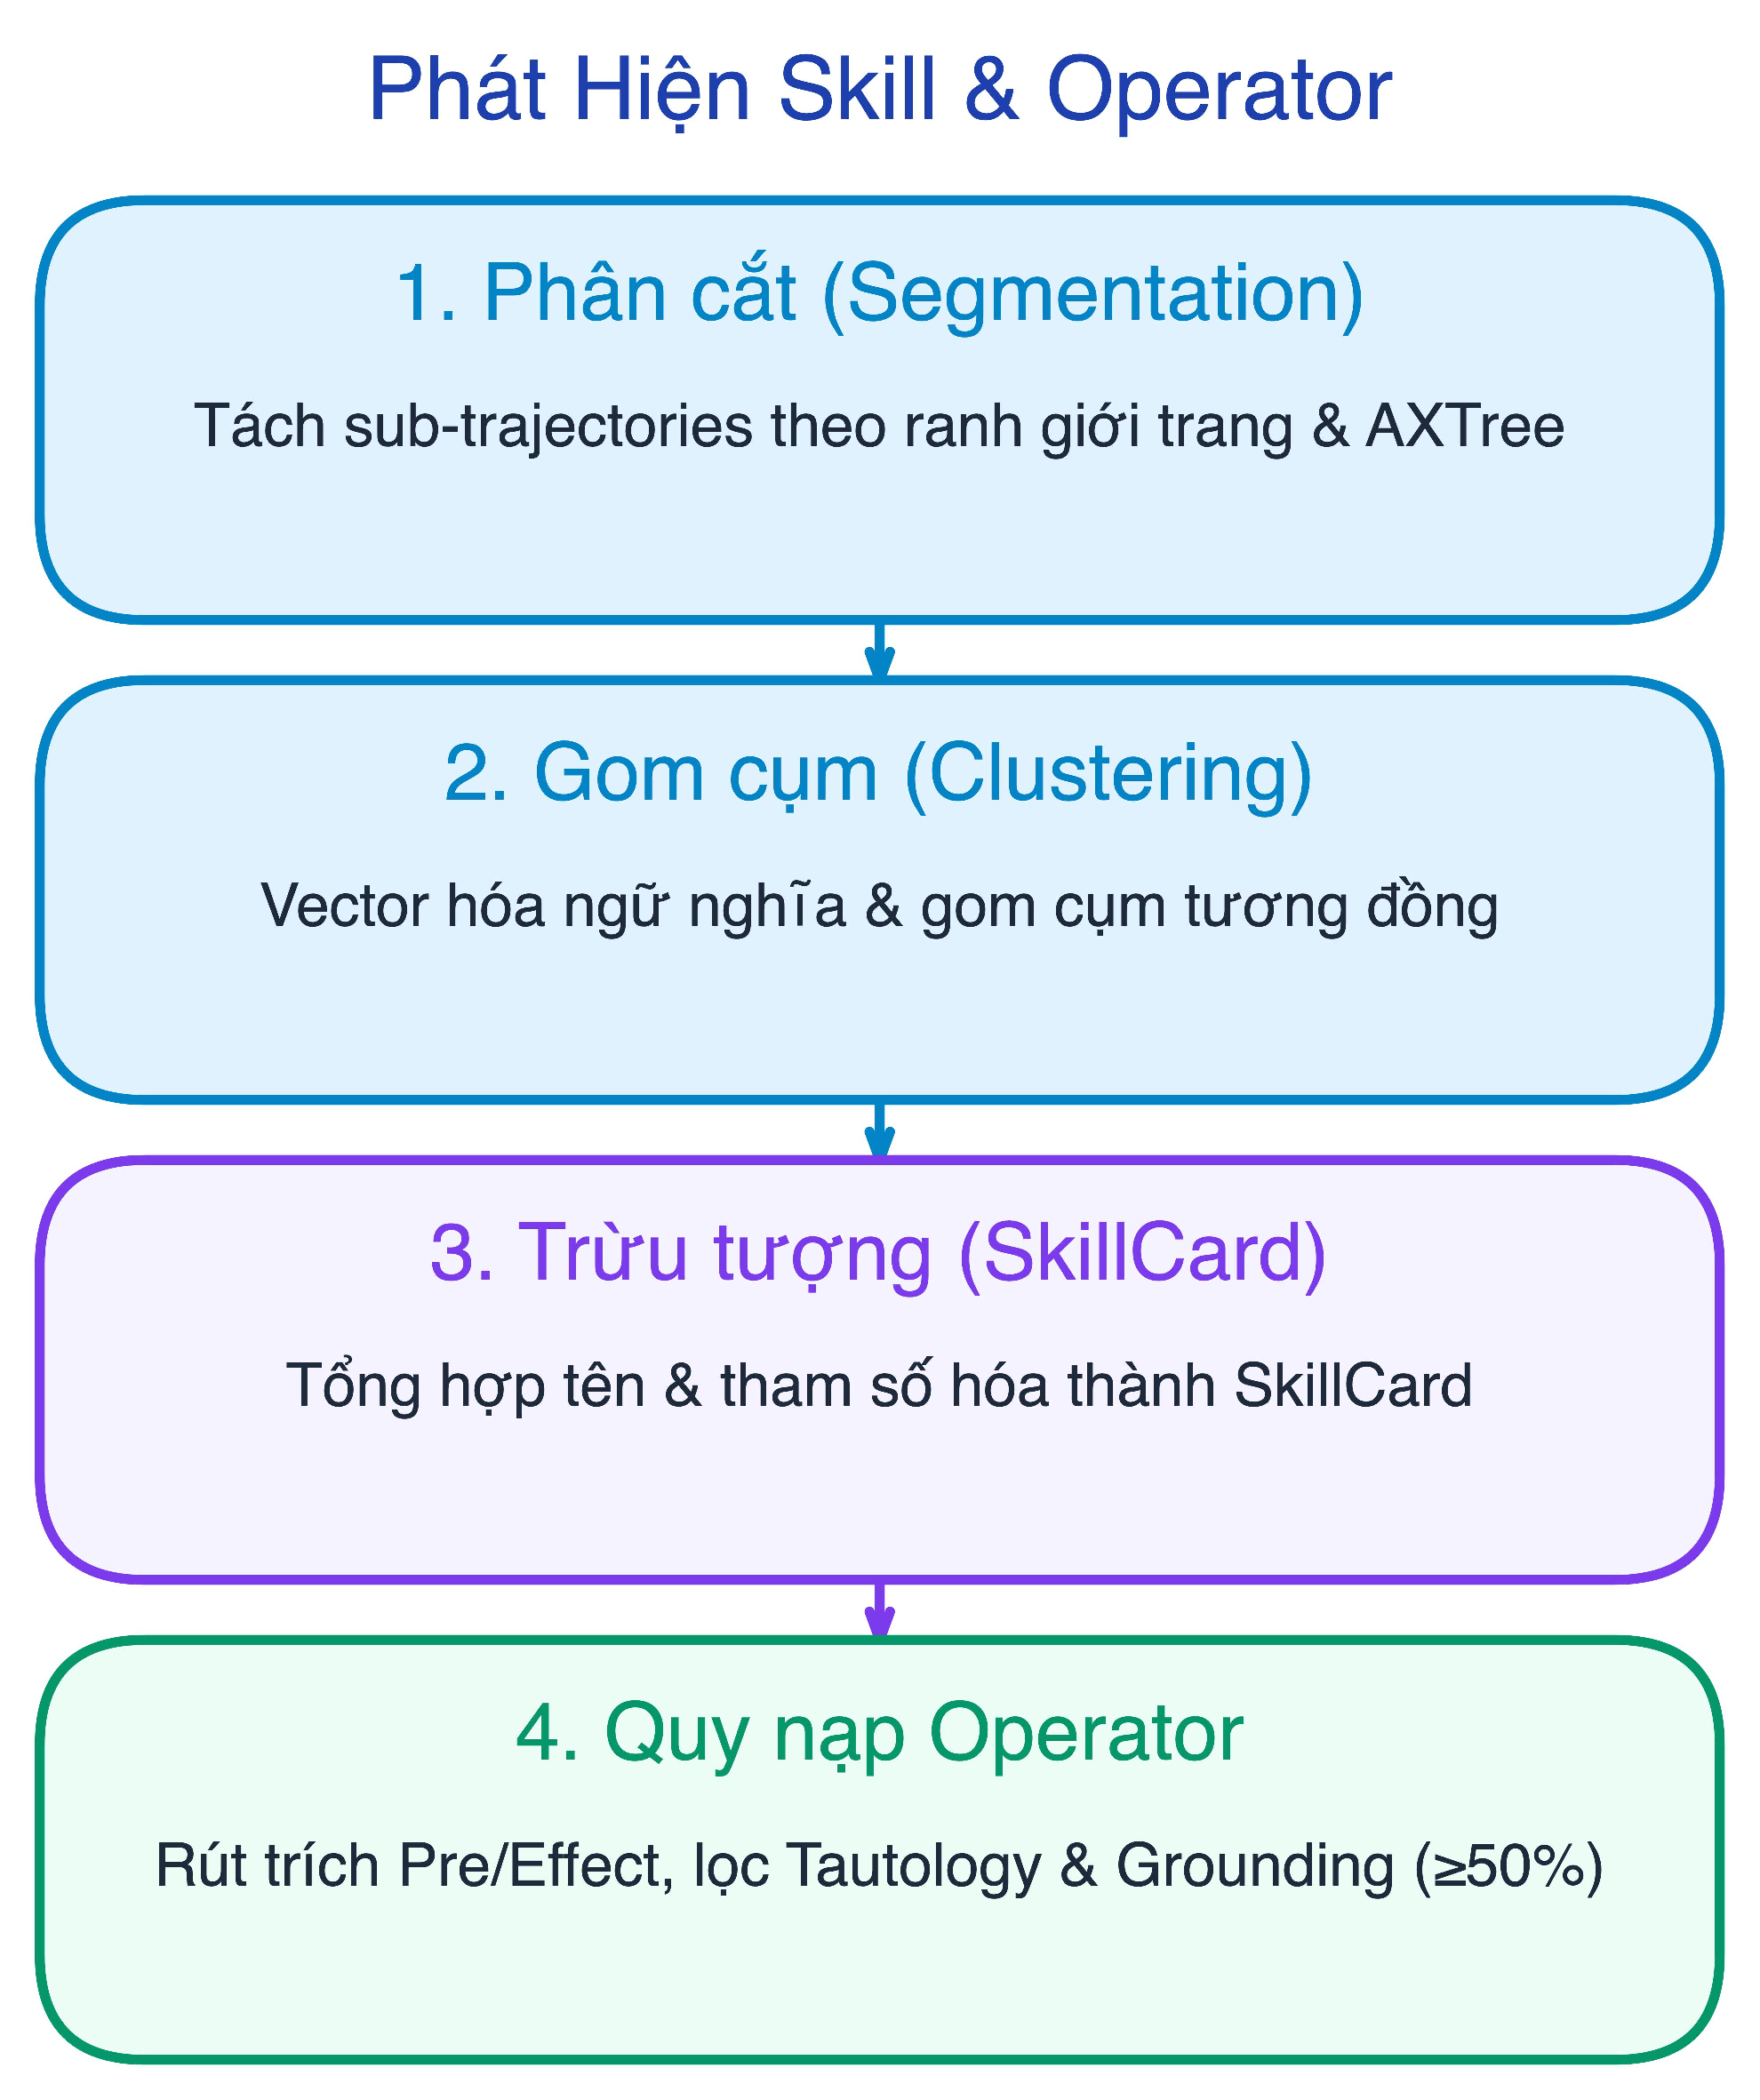
\includegraphics[width=\linewidth,height=0.72\textheight,keepaspectratio]{fig_discovery.pdf}
    \end{column}
    \begin{column}{0.58\textwidth}
      \footnotesize
      Chỉ chạy trên trajectory của task \emph{đã giải thành công}:

      \begin{enumerate}
        \item \textbf{Phân cắt} --- cắt trajectory tại điểm đổi URL và điểm
              tụt độ tương đồng accessibility tree, có LLM trọng tài.
        \item \textbf{Gom cụm} --- clusterer phi tham số theo ngưỡng cosine.
        \item \textbf{Trừu tượng hóa} --- nâng cụm thành \emph{SkillCard}
              có tham số.
        \item \textbf{Kiểm chứng} --- chỉ thu nhận khi lặp lại thành công
              trong ngữ cảnh khác; không đạt thì loại.
      \end{enumerate}

      \vspace{0.15cm}
      \textbf{Skill $\rightarrow$ operator}, hai cổng chặn rút ra từ chạy thật:
      \emph{chống tautology} (effect chỉ lặp lại precondition thì loại) và
      \emph{grounding} (effect không đúng trên $\ge 50\%$ thành viên thì gỡ bỏ).
      Prompt quy nạp \emph{nhận thức từ vựng}: tái dùng nguyên văn mệnh đề đã có,
      vì embedding không hợp nhất được từ đồng nghĩa (0,570 $<$ ngưỡng 0,6).
    \end{column}
  \end{columns}
\end{frame}

\begin{frame}{Sinh semantic task: ghép chuỗi operator}
  \begin{columns}[c]
    \begin{column}{0.60\textwidth}
      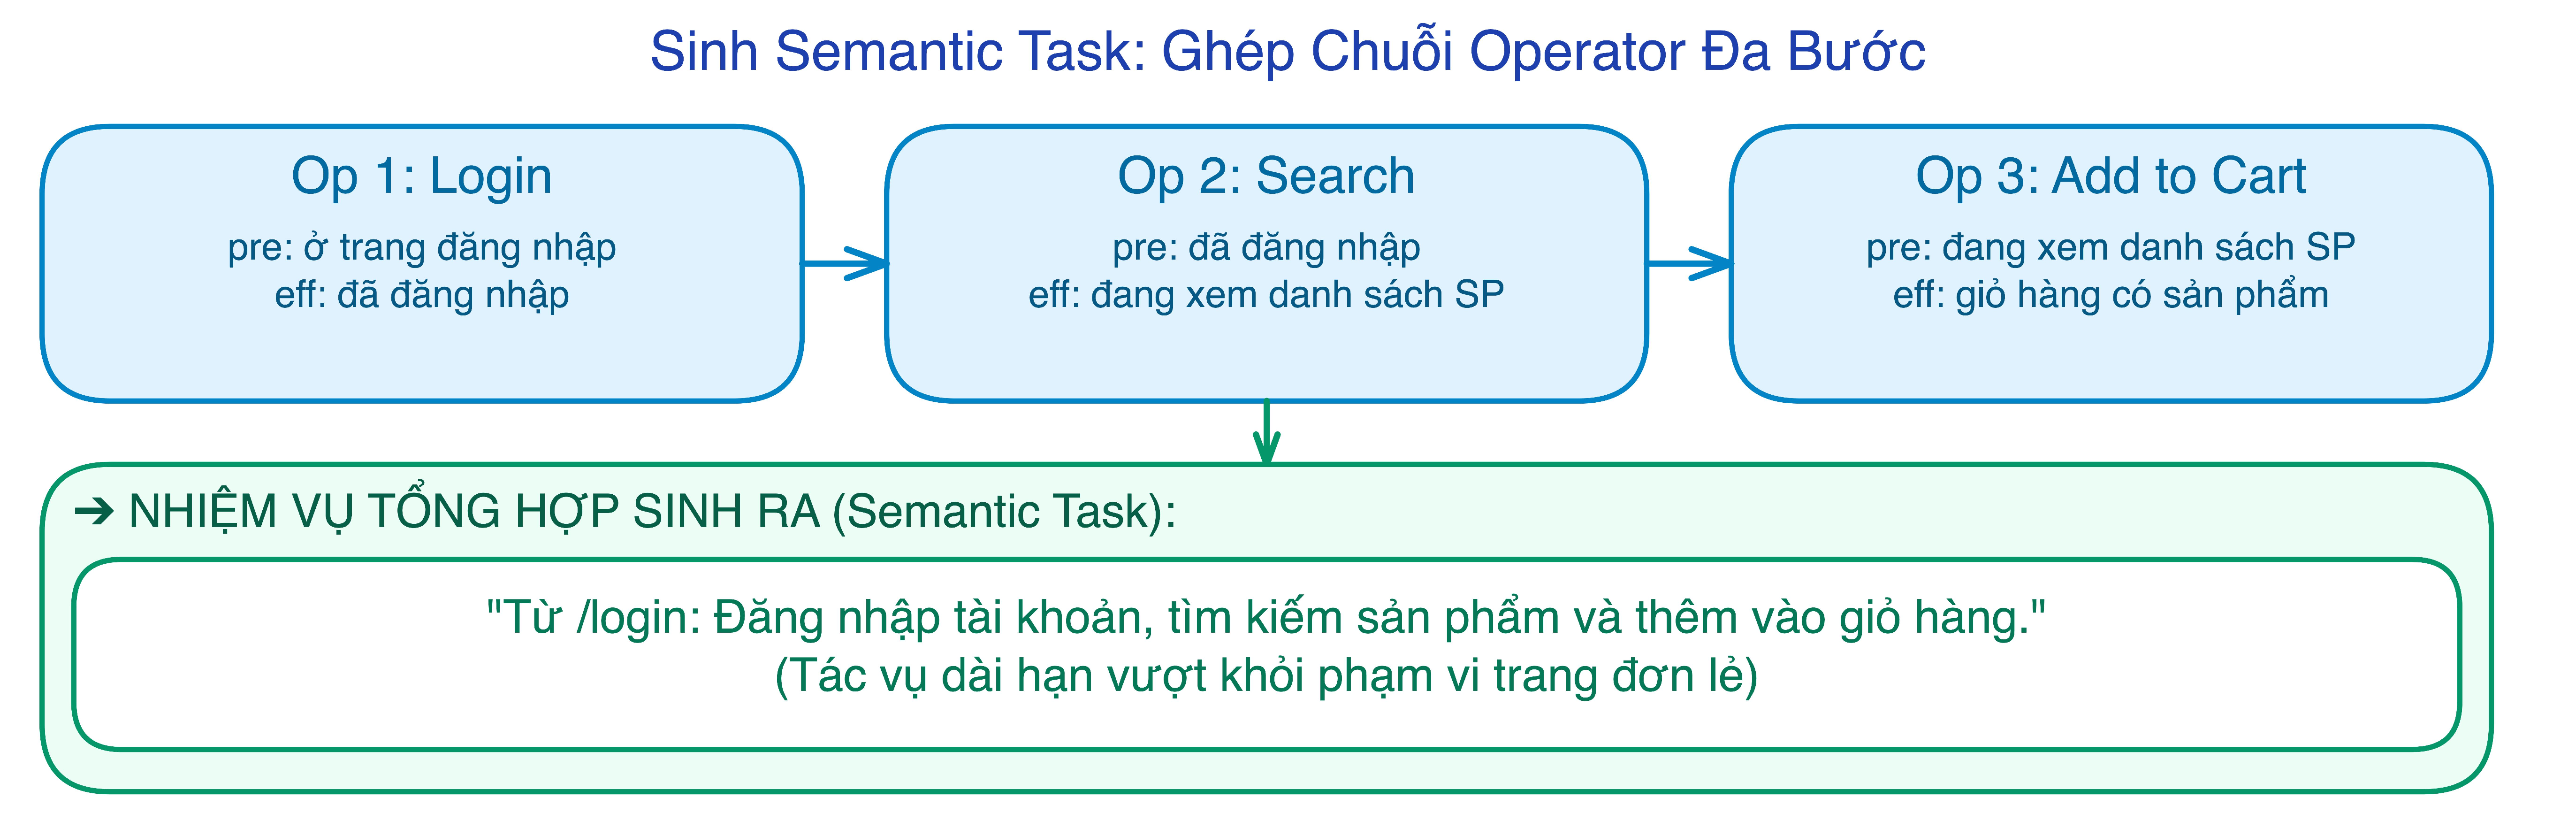
\includegraphics[width=\linewidth,height=0.66\textheight,keepaspectratio]{fig_semantic.pdf}
    \end{column}
    \begin{column}{0.38\textwidth}
      \footnotesize
      Duyệt DFS có chặn trên đồ thị operator: mỗi chuỗi $\ge 2$ operator
      trở thành \emph{một} semantic task nhiều bước, kèm chỉ dẫn sinh từ
      mô tả các skill trong chuỗi.

      \vspace{0.25cm}
      \textbf{Nguồn thứ hai --- seed năng lực website} (từ trên xuống):
      dùng khi đồ thị còn quá thưa để hình thành chuỗi.

      \vspace{0.25cm}
      \textit{Thực tế đo được:} 66 semantic task đã thực thi, chia thành
      \kw{59 từ seed} và \kw{7 từ ghép chuỗi} --- cơ chế từ dưới lên chạy
      \emph{đúng thiết kế nhưng thưa}; nguyên nhân được phân tích ở Chương 5.
    \end{column}
  \end{columns}
\end{frame}

\begin{frame}{Tinh lọc dữ liệu và nguyên tắc prompt parity}
  \begin{columns}[c]
    \begin{column}{0.32\textwidth}
      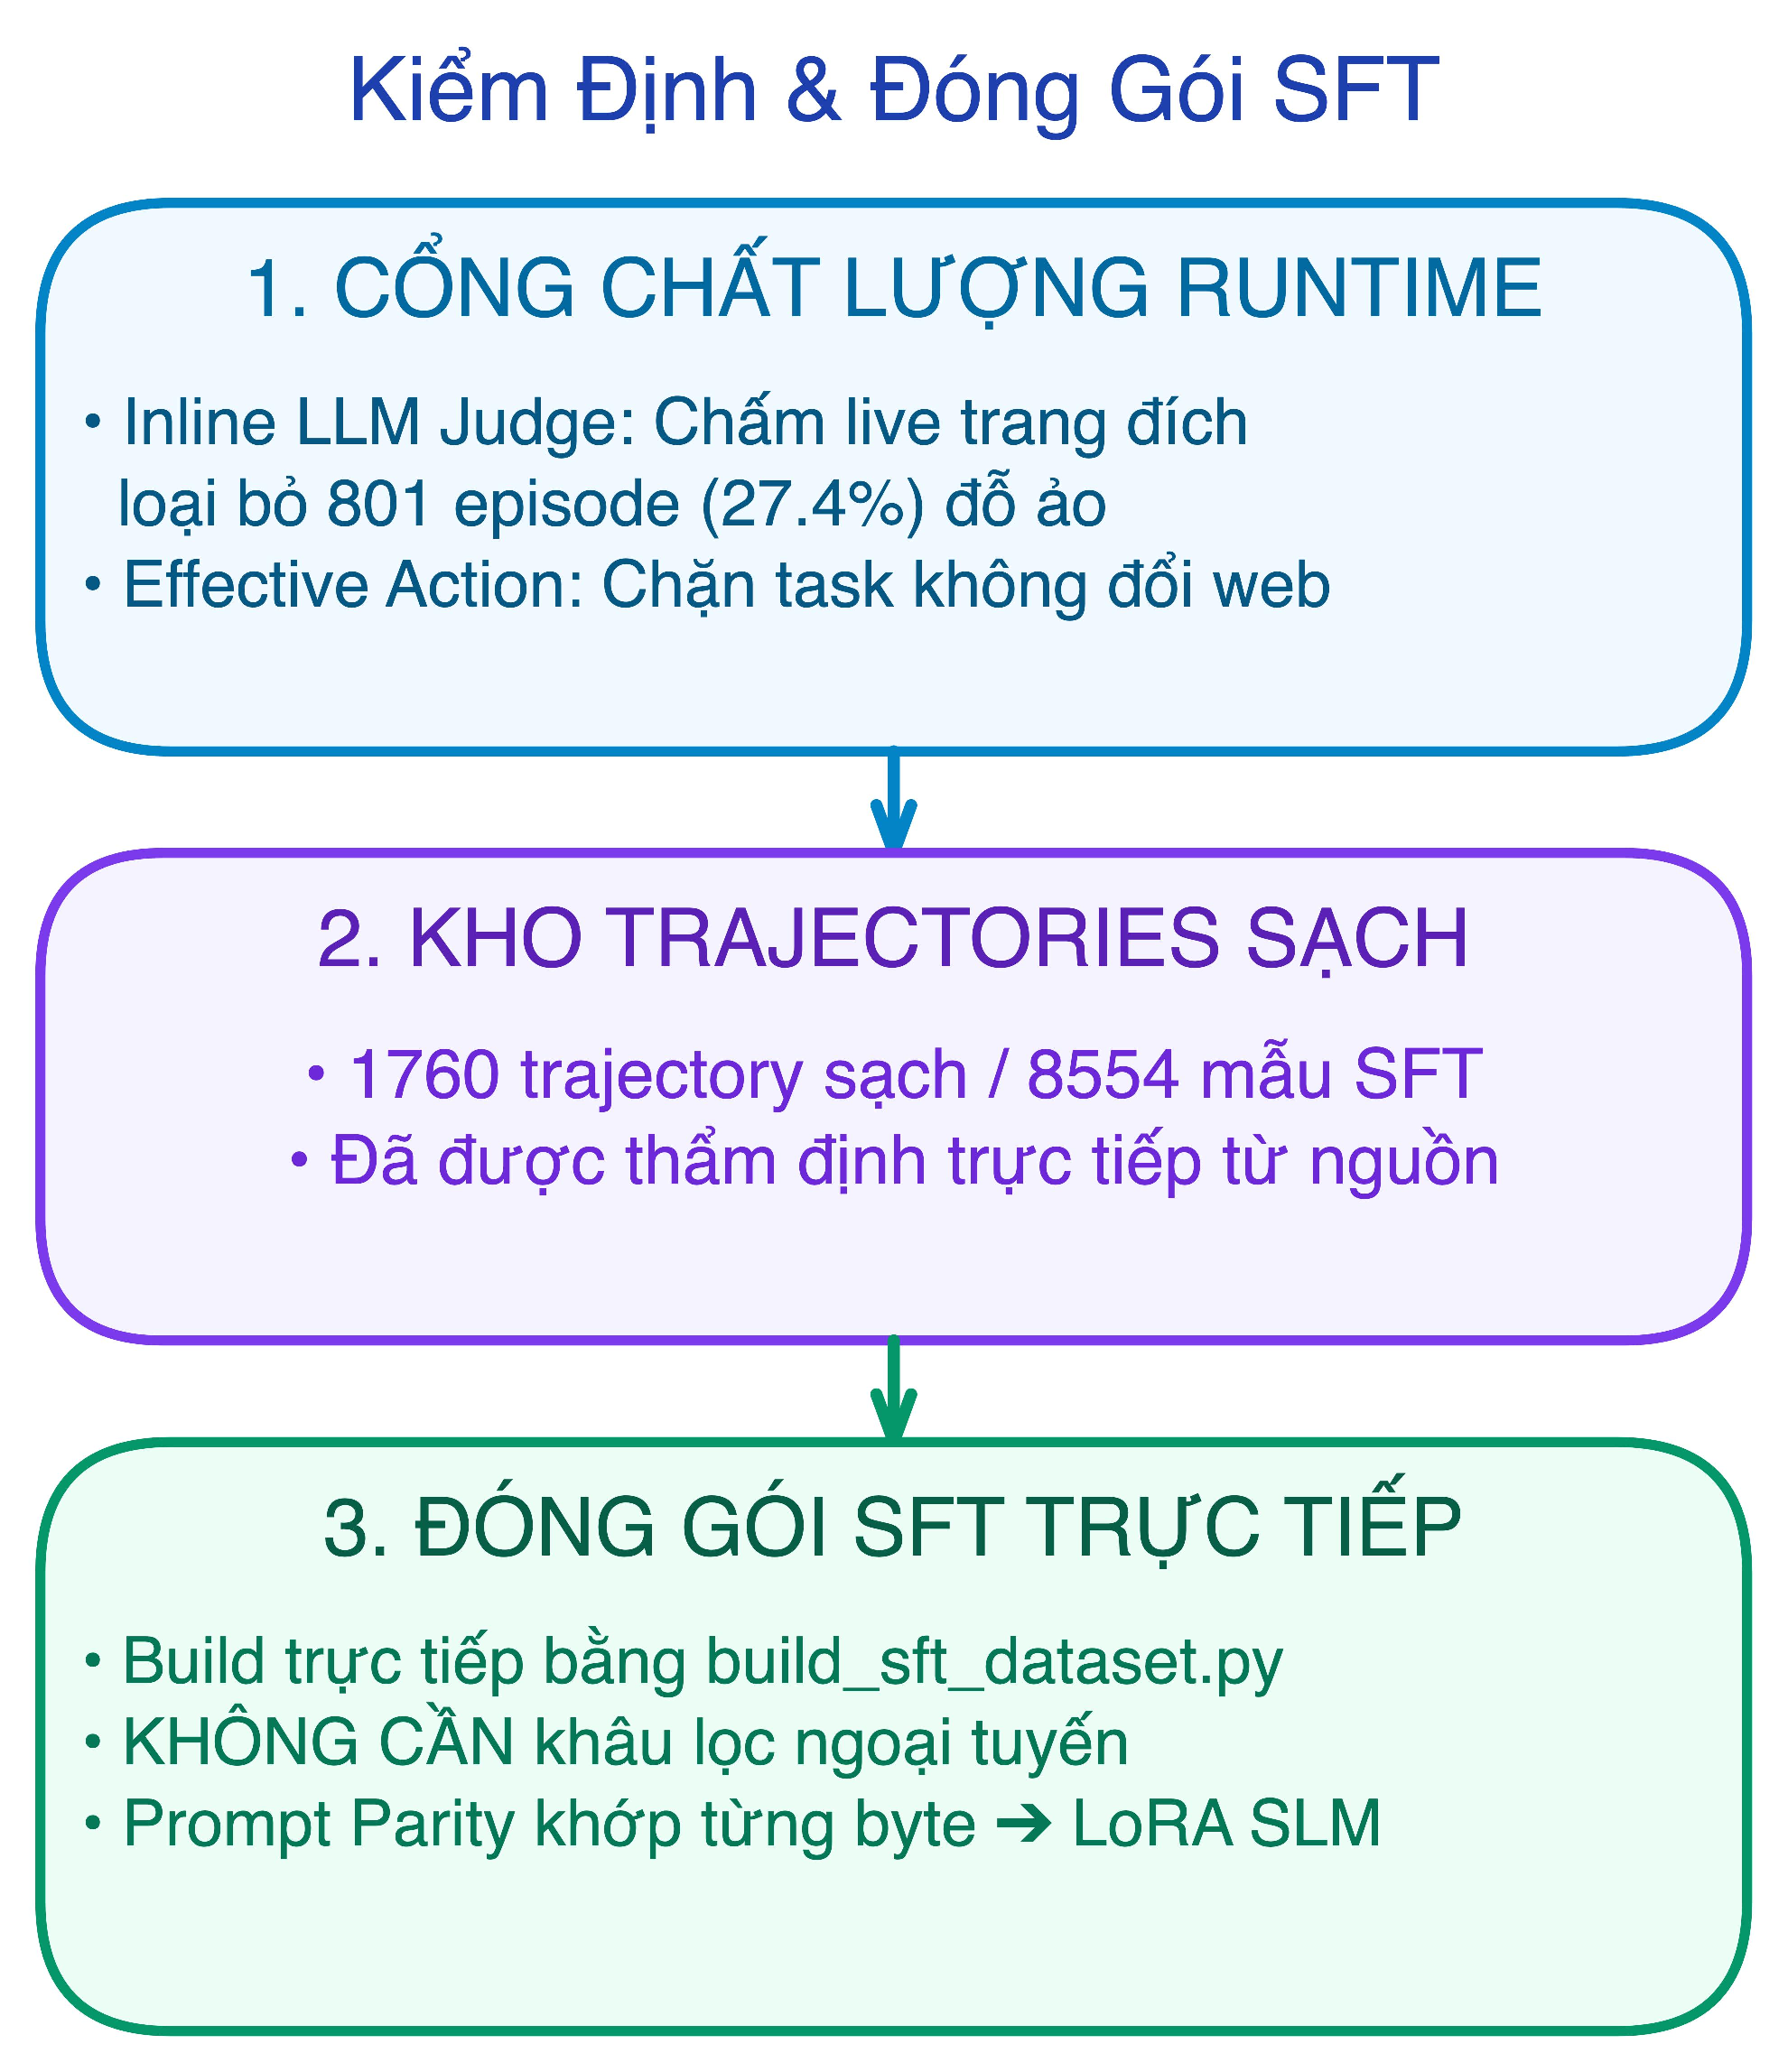
\includegraphics[width=\linewidth,height=0.74\textheight,keepaspectratio]{fig_curation.pdf}
    \end{column}
    \begin{column}{0.66\textwidth}
      \footnotesize
      \textbf{Không episode nào được tính thành công bằng lời khai của agent.}

      \begin{itemize}
        \item \textbf{Cổng chấm lại (judge)} --- mọi lần agent tự tuyên bố hoàn
              thành đều được một LLM độc lập chấm lại trên chính trang cuối.
              Đã hạ cấp \kw{497 episode ($\approx$32\%)}.
        \item \textbf{Cổng hành động hữu hiệu} --- task \texttt{[MOD]}/\texttt{[NAV]}
              mà không có hành động nào thay đổi trang thì bị loại: một task
              ``sửa đổi'' không sửa gì là thành công giả. Loại thêm
              \kw{104 trajectory}. Judge \emph{không} bắt được nhóm này vì
              trang cuối không hề đổi.
        \item \textbf{Viết lại suy nghĩ} --- trạng thái, phản tư, subgoal,
              kiểm tra hoàn thành.
      \end{itemize}

      \vspace{0.15cm}
      \textbf{Prompt parity:} prompt huấn luyện \emph{trùng từng byte} với prompt
      solver dùng lúc chạy thật, kể cả ngưỡng cắt accessibility tree 6000 ký tự.
      Chia train/val ở cấp \emph{task} $\rightarrow$ \kw{0} mục tiêu trùng nhau
      giữa hai tập.
    \end{column}
  \end{columns}
\end{frame}
